% !TEX root = ../main.tex

\subsection{The Rust Programming Language} % (fold)
\label{sub:the_rust_programming_language}

Rust \cite{web:rust_lang} is a new open source systems programming language developed by the Mozilla
Foundation \cite{web:mozilla_foundation}. It is designed to support concurrency and parallelism and
take full utilization of the underlying hardware. Rust makes strong guarantees about isolation and
memory safety, while still focusing on performance.

\subsubsection{Language Features} % (fold)
\label{ssub:language_features}

Rust is a strongly and statically typed, multi-paradigm programming language. The language borrows
many traits and features from other, already existing languages. The following subsections discusses
some of the more prominent language features, that all work together in order to achieves Rust's
main goals; mainly full memory safety without sacrificing performance.
\todo{I've just been throwing out ideas and statements that are probably not very true.}

\paragraph{Guaranteed memory safety} \hfill

One of rusts biggest features is full memory safety \cite{web:rust_book_unsafe}

\paragraph{Zero-cost Abstractions} \hfill

Abstractions, in the form of references and pointers to objects or structures and how they are
structured on the heap, is a common source of overhead in programming languages.
\autoref{fig:java_abstractions} \todo{Update with nicer figure} shows how Java lays out a vector of
strings in memory. A reference to the heap-allocated vector is placed on the stack, and the vector
itself stores internal references to different strings that is placed elsewhere on the heap. Thus,
if the programmer wants to access the first character of a string, two objects have to be found and
dereferenced on the heap in order to read the value;

\begin{enumerate}
  \item the vector must be dereferenced so that a reference to the string can be returned, and
  \item the string must be dereferenced so that character can be read.
\end{enumerate}

If the nesting of objects is deep it can result in many unnecessary heap-lookups in order to get the
desired data.

\begin{figure}[tb]
  \begin{center}
    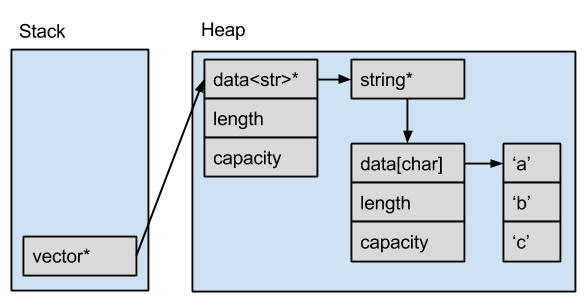
\includegraphics[scale=0.5]{figures/java_abstractions}
  \end{center}
  \caption{Abstractions of a Vector of Strings in Java.}
  \label{fig:java_abstractions}
\end{figure}

Rust introduces the same zero-cost abstractions that are featured in C and C++, among others. This
is both important for performance, and generally in order to have a deterministic and a common
understanding of how the structures are laid out in the memory when working with embedded devices.
\todocite{This is a bogus sentence. Also, need to cite zero-cost abstraction articles}
\autoref{fig:cpp_abstractions} shows how C++ places the structures in memory. The main difference
is that the structure data itself is placed on the stack and inside the vector, instead of the
references to the structures, yet keeping the same level of abstraction. In Rust's case, all
structures is allocated directly on the stack if it is not shared between threads (see the following
paragraphs), allowing for faster data access. This is made possible with a strong notion of variable
ownership in order for the compiler to statically keep track of live stack- and heap-references.
\todo{Don't think this last section is entirely true. Leaving this as a statement for now, that
needs proper backing.}

\begin{figure}[tb]
  \begin{center}
    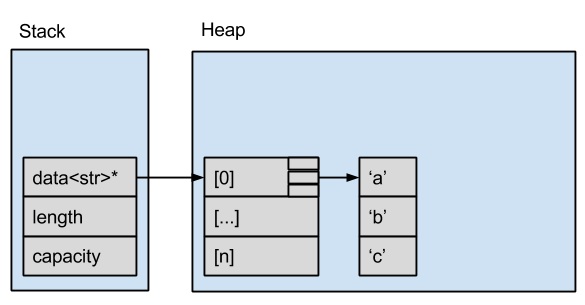
\includegraphics[scale=0.5]{figures/cpp_abstractions}
  \end{center}
  \caption{Abstractions of a Vector of Strings in Rust and C++.}
  \label{fig:cpp_abstractions}
\end{figure}



\paragraph{Ownership and Move Semantics} \hfill

\paragraph{Big-Stack allocation} \hfill
\label{par:big_stack}

Rust uses "big stack" allocations \todocite{need big-stack citation. I've read about it somewhere}
and does a good job of avoiding dynamic heap allocation of data. Combined with Rust's strong
lifetime semantics, it is possible to write larger programs that are fully stack-allocated, with
little or no dynamic heap allocations. This can significantly boost performance as the need for
garbage collectors and other runtime requirements is minimal (important for embedded devices).

\todo{Just rambling along to get an idea of something to write.}

% subsubsection language_features (end)

\subsubsection{Memory Safety} % (fold)
\label{ssub:memory_safety}

Rust makes strong guarantees about memory safety.

% subsubsection memory_safety (end)

\subsubsection{Concurrency Model} % (fold)
\label{ssub:concurrency_model}

Rust has a concurrency model. Duh.

% subsubsection concurrency_model (end)



% subsection the_rust_programming_language (end)
